\section{Wahrscheinlichkeitsverteilung}

\subsection{Kumulative Häufigkeitsverteilung}

\begin{minipage}{0.38\columnwidth}
	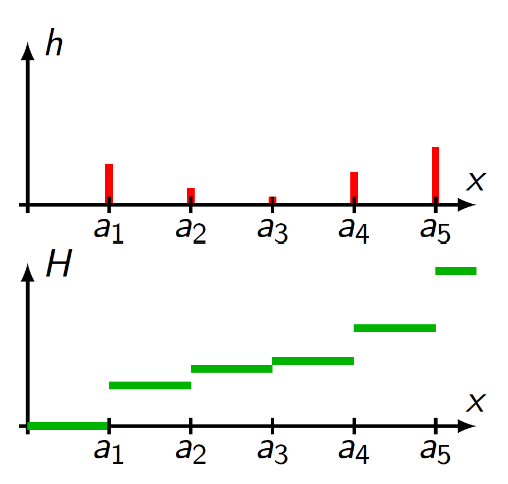
\includegraphics[width=\columnwidth]{images/kumulativeHaufigkeitsverteilung.png}
\end{minipage}
\hfill
\begin{minipage}{0.6\columnwidth}
	$$ H_j  = \sum\limits_{k=1}^j  h_k = | \{ x_i | x_i \leq a_j \} | $$
	$=$ Anzahl Merkmalsausprägungen 'links von $a_j$'
	
	\vspace{0.2cm}

	Allgemeiner:
	$$ H(x) = | \{ i | x_i \leq x \} | $$
	Stückweise konstant, Sprungstellen bei $a_j$ \\
	\textbf{Sprunghöhe} \crd{$h_j$}
\end{minipage}


\subsubsection{Relative Häufigkeit}

Maximum von $H(x)$ hängt von $n$ ab \textrightarrow relative Häufigkeit verwenden:

\begin{minipage}[c]{0.3\columnwidth}
	$$ f_j = \frac{1}{n} h_j $$
\end{minipage}
\hfill
\begin{minipage}[c]{0.3\columnwidth}
	$$ F_j = \frac{1}{n} H_j $$
\end{minipage}
\hfill
\begin{minipage}[c]{0.3\columnwidth}
	$$ F(x) = \frac{1}{n} H(x) $$
\end{minipage}


\subsection[Verteilungsfunktion]{Verteilungsfunktion $\bm{F}$}

\textbf{Definiton:}
Ist $X$ einer Zufallsvariable, so ist die Verteilungfunktion von $X$ definiert als
$$ \boxed{ F(x) = F_X(x) = P(X \leq x) } $$ 
Die Verteilungsfunktion beschreibt die \textbf{Wahrscheinlichkeit der Werte} einer Zufallsvariablen

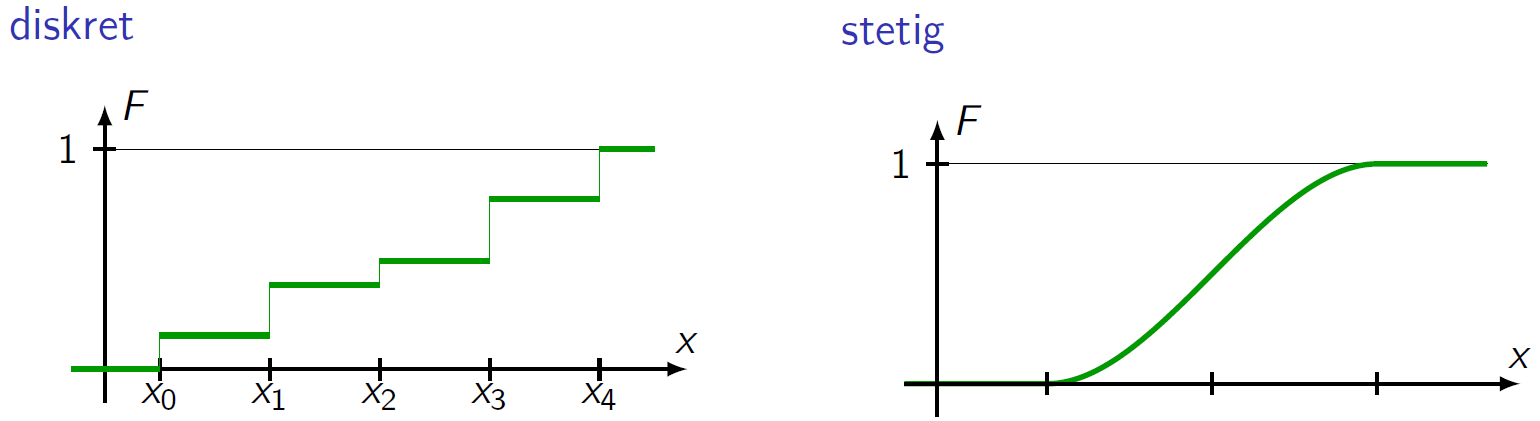
\includegraphics[width=0.9\columnwidth]{images/Verteilungsfunktion.png}


\subsubsection{Eigenschaften der Verteilungsfunktion}

\begin{itemize}
	\item $ F_X(x) $ ist monoton wachsend 
	\item $ 0 \leq F_X(x) \leq 1$ 
	\item $ \lim \limits_{x \to - \infty } F(x) = 0, \lim\limits_{x \to \infty} F(x) = 1 $ 
\end{itemize}

\vspace{0.2cm}

\begin{minipage}[t]{0.42\columnwidth}
	\begin{center}
		\myul{\textbf{Wahrscheinlichkeit für Intervall}}
		$$ \boxed{ P(a < X \leq b) = F_X(b) - F_X(a) } $$
	\end{center}
\end{minipage}
\hfill
\begin{minipage}[t]{0.55\columnwidth}
	\begin{center}
		\myul{\textbf{'Umkehrung'}}
		$$ \boxed{ P(X \leq x) = F(x) \text{ \textlrarrow\ } P( X > x) = 1 - F(x) } $$ 
	\end{center}
\end{minipage}


\subsubsection{Berechnung der Verteilungsfunktion}

Die Verteilungsfunktion $F(x) = P(X \leq x) $ ist eine Wahrscheinlichkeit 

\vspace{0.1cm}

\begin{enumerate}
	\item Fragen über $F(x)$ in Wahrscheinlichkeit von Ergebnissen übersetzen. 
	\item Rechenregeln für Wahrscheinlichkeit anwenden
	\item Wahrscheinlichkeit durch $F(x)$ ausdrücken, rückübersetzen 
\end{enumerate}


\example{Maximum zweier Zufallsvariablen}

\vspace{-0.2cm}

\begin{minipage}[c]{0.5\columnwidth}
	\textbf{Gegeben}\\
	Zwei unabh. Zufallsvariablen $X$ und $Y$ mit Verteilungsfunktion $F_X(x)$ und $F_Y(y)$
	\vspace{0.2cm}

	\textbf{Gesucht} \\
	Verteilungsfunktion $F_{\mathrm{max}(X,Y)}(x) = F_Z(z)$ 
\end{minipage}
\hfill
\begin{minipage}[c]{0.4\columnwidth}
	\begin{align*}
		F_Z(z)	&= P(Z  \leq z) 					\\
				&= P(\mathrm{max}(X,Y) \leq z) 		\\
				&= P(X \leq z \wedge  Y \leq z) 	\\
				&= P(X \leq z) \cdot P(Y \leq z) 	\\
		F_Z(z) 	&= F_X(z) \cdot F_Y(z)
		\end{align*} 
\end{minipage}


\subsubsection{Verteilungsfunktion des Maximums}

$X_1$ und $X_2$ sind zwei gleichverteilte Zufallsvariablen (z.B. Würfel)

\vspace{0.2cm}

Verteilungsfunktion von $F_{\mathrm{max}(X_1 ,X_2)}(x) = F_{X_1} (x_1)^2 = F_{X_2}(x_2)^2 $

\begin{center}
	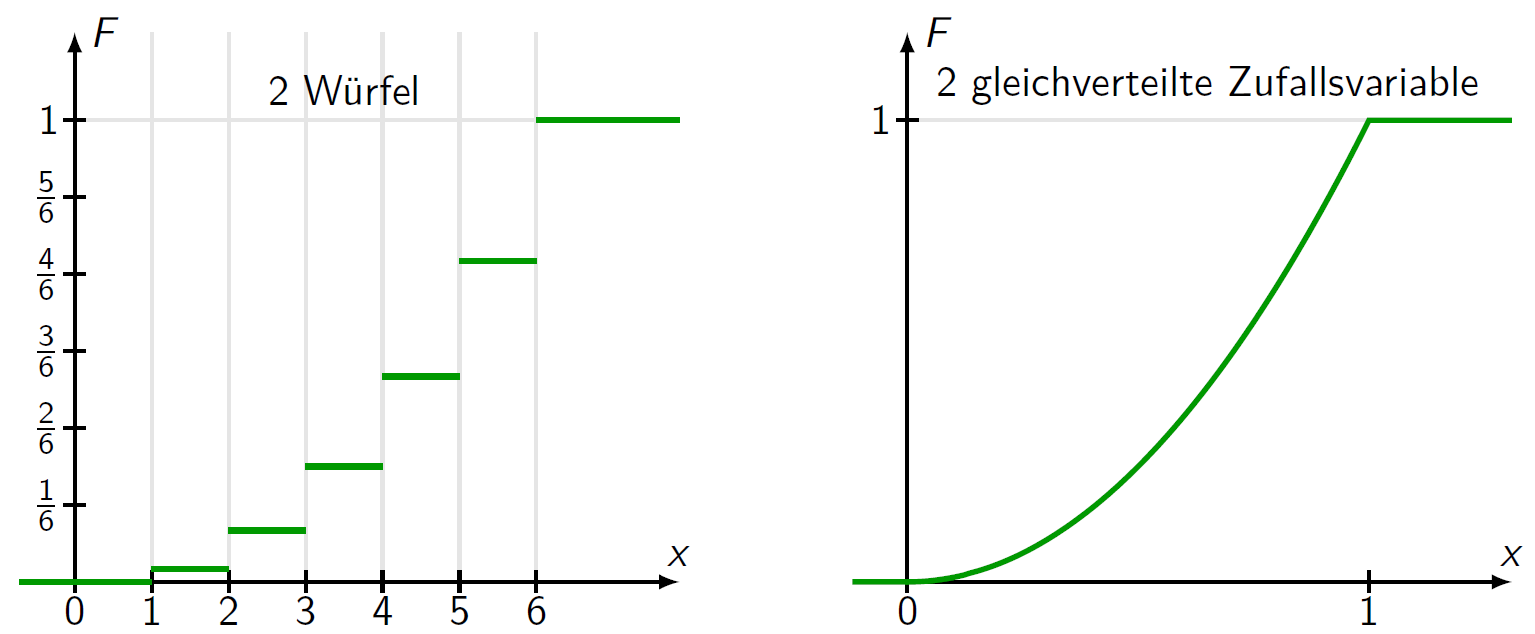
\includegraphics[width=0.8\columnwidth]{images/VerteilungsfunktionDesMaximums.png}
\end{center}


\subsection{Wichtige Werte in einem Diagramm}

\myul{\textbf{Mittelwert}}

\begin{minipage}[t]{0.48\columnwidth}
	$$ \boxed{ \crd{\overline{x}} = \frac{1}{n} \sum\limits_{i=1}^n x_i } $$
\end{minipage}
\hfill
\begin{minipage}[t]{0.48\columnwidth}
	$$ \boxed{ \text{minimiert: }  \sum\limits_{i=1}^n (x_i - \crd{\overline{x}})^2 } $$
\end{minipage}

\vspace{0.3cm}

\myul{\textbf{Gewichteter Mittelwert}}

\begin{minipage}[t]{0.48\columnwidth}
	$$ \boxed{ \crd{\overline{x}} = \frac{\sum\limits_{i=1}^n w_i \, x_i }{\sum\limits_{i=1}^n w_i } } $$
\end{minipage}
\hfill
\begin{minipage}[t]{0.48\columnwidth}
	$$ \boxed{ \text{minimiert: }  \sum\limits_{i=1}^n w_i \, (x_i - \crd{\overline{x}})^2 } $$
\end{minipage}

\vspace{0.3cm}

\begin{minipage}[t]{0.48\columnwidth}
	\raggedright
	\myul{\textbf{Median}}

	\vspace{0.1cm}

	Mittlerer Wert / 0.5-Quantil \\
	(Mittelwert der beiden mittleren Werte falls $n$ gerade ist) 

	\begin{center}
		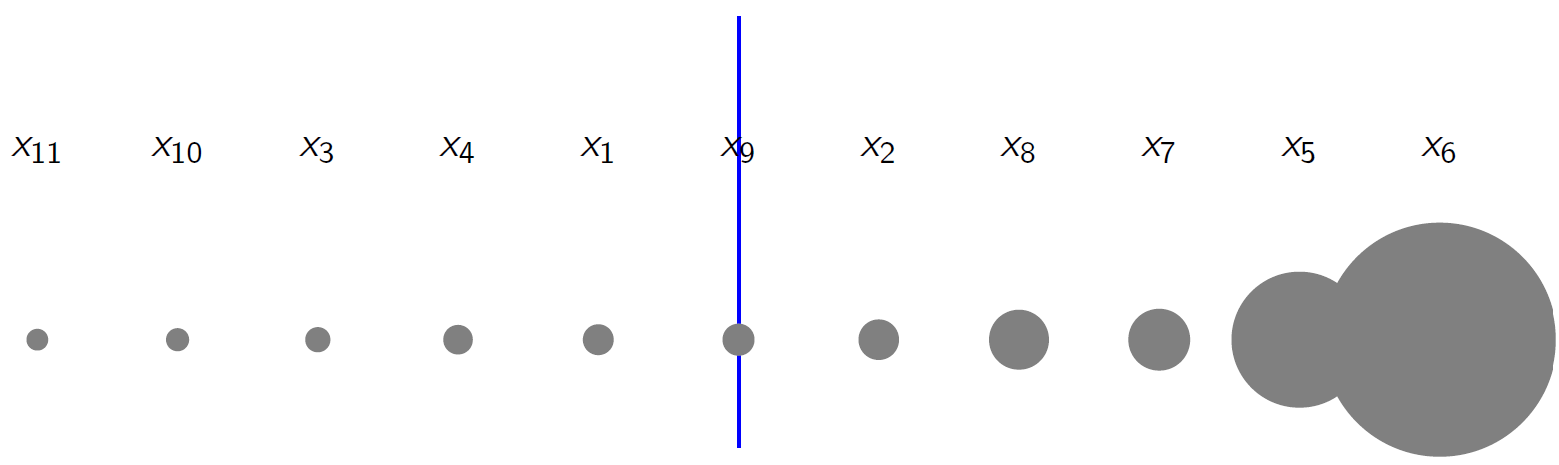
\includegraphics[width=0.9\columnwidth]{images/median.png}
	\end{center}
\end{minipage}
\hfill
\begin{minipage}[t]{0.48\columnwidth}
	\raggedright
	\myul{\textbf{Modus / Modalwert}}

	\vspace{0.1cm}

	Häufigster Wert

	\begin{center}
		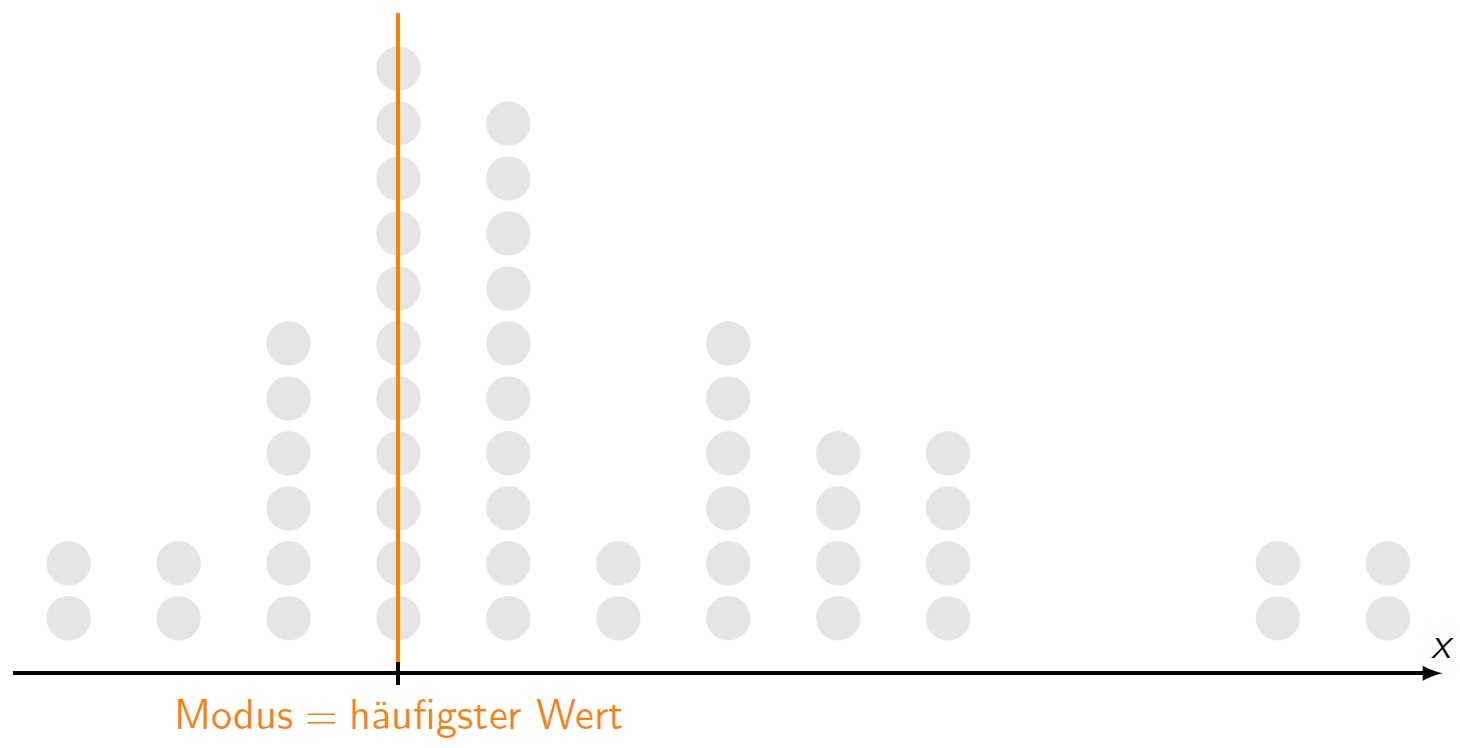
\includegraphics[width=0.85\columnwidth]{images/modus.png}
	\end{center}
\end{minipage}

\vspace{0.3cm}

\myul{\textbf{Spannweite $\bm{R}$ / Quartilabstand $\bm{Q}$}}

\begin{center}
	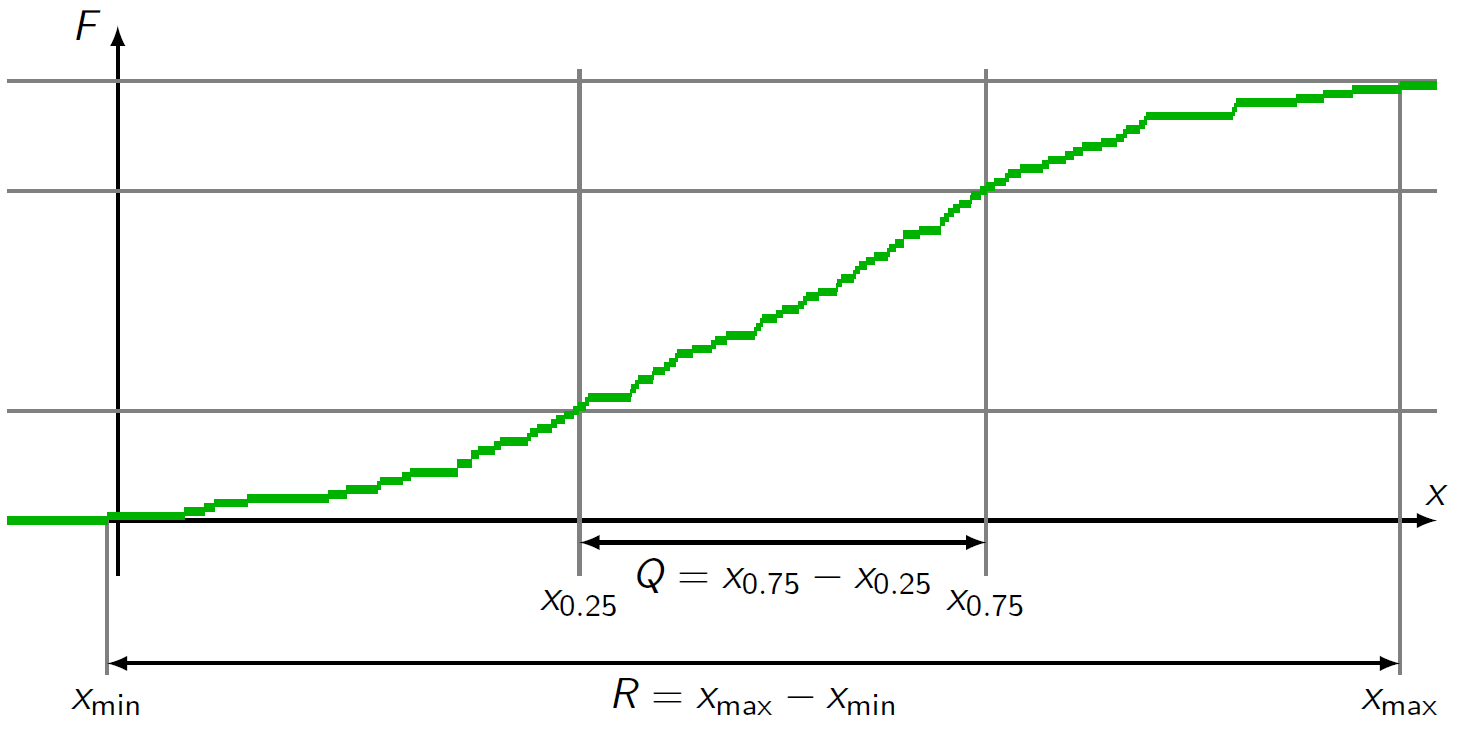
\includegraphics[width=0.65\columnwidth]{images/spannweite_quartilabstand.png}
\end{center}


\subsection[Wahrscheinlichkeitdichte]{Wahrscheinlichkeitdichte $\bm{\varphi(x)}$}

\textbf{Achtung: Nur für stetige Zufallsvariablen}

\vspace{0.2cm}

\begin{minipage}{0.33\columnwidth}
	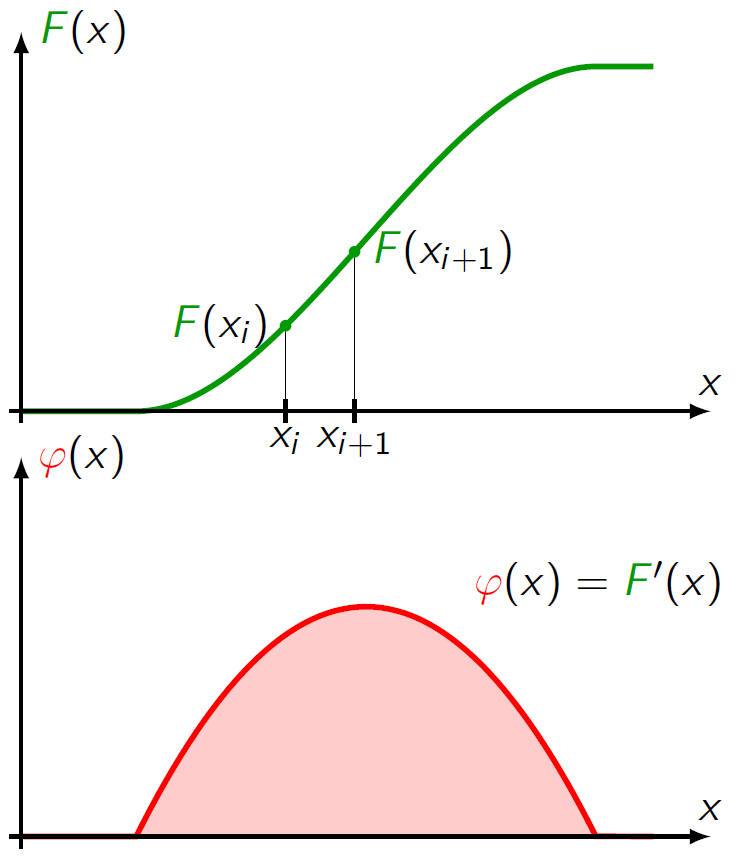
\includegraphics[width=\columnwidth]{images/wahrscheinlichkeitsdichte_1.png}
\end{minipage}
\hfill
\begin{minipage}{0.6\columnwidth}
	\myul{ \textbf{Eigenschaften von $\crd{\varphi}(x)$} }

	\vspace{0.1cm}

	\begin{itemize}
		\item $\crd{\varphi}(x) = \cgn{F}'(x)$
		\item $P(a < X \leq b) = \int\limits_a^b \crd{\varphi}(x) \, \diff x $
		\item $\cgn{F}(x) = \int\limits_{-\infty}^x \varphi(\xi) \, \diff \xi$
		\item $\int\limits_{-\infty}^{\infty} \varphi(x) = 1$ (Normierungsbedingung)
		\item $\varphi(x) \geq 0 \quad \forall \, x \in \mathbb{R}$
	\end{itemize}
\end{minipage}

$$ \varphi_{X+Y}(x) = (\varphi_X * \varphi_Y)(x) = \int\limits_{-\infty}^{\infty} \varphi_X(t) \cdot \varphi_Y(x - t) \, \diff t \quad \text{(Faltung)} $$


\subsection{Erwartungswert mittels Wahrscheinlichkeitsdichte}

\vspace{-0.2cm}
\begin{align*}
	E(\cgn{X})		&= \cbl{\sum} \cgn{\text{Wert}} \times \crd{\text{Wahrscheinlichkeit}} 					\\
					&= \cbl{\int\limits_{-\infty}^{\infty}} \cgn{x} \cdot \crd{\varphi(x) \, \diff x}  		\\
	E(\cgn{X^2}) 	&= \cbl{\int\limits_{-\infty}^{\infty}} \cgn{x^2} \cdot \crd{\varphi(x) \, \diff x} 	\\
	E(\cgn{f(x)}) 	&= \cbl{\int\limits_{-\infty}^{\infty}} \cgn{f(x)} \cdot \crd{\varphi(x) \, \diff x} 
\end{align*} 


\example{Bestimmung $\bm{E(X)}$ im Intervall [a, b]}

\begin{enumerate}
	\setlength\itemsep{1em}

	\item Normierungsbedingung überprüfen \quad $\int\limits_{- \infty}^{\infty} \varphi(x) \, dx \overset{!}{=} 1$
	\item Erwartungswert $E(X)$ bestimmen \quad $E(X) = \int\limits_{-\infty}^{\infty} x \cdot \varphi(x) \, \diff x$
	\item $E(X^2)$ berechnen \quad $E(X^2) = \int\limits_{-\infty}^{\infty} x^2 \cdot \varphi(x) \, \diff x$
	\item Varianz berechnen \quad $\sigma^2 = \var(x) = E(X^2) - E(X)^2$
	\item Wurzel der Varianz berechnen (und ev. einzeichnen)
\end{enumerate}

